\documentclass[a4paper, 10pt]{scrartcl}
\usepackage{amsmath}
\usepackage{graphicx}
\usepackage[colorlinks]{hyperref}
\usepackage{typearea}
\typearea{12}
\makeatletter
\newcommand{\figcaption}[1]{\def\@captype{figure}\caption{#1}}
\newcommand{\tblcaption}[1]{\def\@captype{table}\caption{#1}}
\makeatother
\begin{document}

\title{Comparison of 7m-array observations with ACACORR and BLC: CSV-3664 HH114MMS}
\author{Seiji Kameno, Jennifer Donovan Meyer, Antonio Hales}
% \date{\today}
\maketitle
\begin{abstract}
Here are comparison of Band-3 7m-array mosaic observations correlated by the baseline correlator (BLC) and ACA correlator (ACAC).
We have run two ExecBlocks with ACAC and BLC consequently near the transit of the target source HH114MMS to minimize the differences in $(u, v)$ coverage.
The results in continuum flux density and line profiles are almost consistent within the difference $<5.2$\%, except one line species.
We consider the difference would be caused by coarse spectral sampling and channel mis-alignment between two executions.
\end{abstract}

\section{Introduction}
CSV-3664 is to verify the consistency of 7m-array executions with both BLC and ACAC. The purpose is to enable contingency in case the ACAC stops working due to hardware problems or decommission.
We have reported the initial comparison results of Band-6 observations in \href{http://www.alma.cl/~skameno/Documents/CSV-3664/}{CSV-3664 report}. There, most of results are consistent between two correlators, except strong emission lines that required renormalization correction.

\section{Methods: Science SB executions on 2022-05-22}
Here we report about Band-3 mosaic observations toward weak line source, HH114MMS. Two executions with ACAC and BLC were carried out straddling the transit, to obtain similar $(u,v)$ coverage.
Executions are listed in tables \ref{tab:EBlist}. Two executions with equivalent SBs. Both SBs were generated using the same SG, but one was generated for the BLC and the other for the ACAC.

Standard data reduction with CASA (version PIPELINE 6.2.1.7) has been carried out to produce image cubes of two targets.
Standard amplitude calibration, bandpass calibration, phase calibration processes were applied.

For BLC, $T_{\mathrm{sys}}$ spectra are acquired in TDM SPWs which has a coarser spectral resolution than FDM SPWs, while ACAC employs the common spectral setup for both atmCal and interferometry scans.
Flux scaling was applied using J0423-0120 as the flux calibrator.
See the reduction script \href{https://jira.alma.cl/secure/attachment/457290/HH114.py}{HH114.py}.
Note that the reduction procedure does NOT contain non-standaard calibration processes such as renormalization steps.

\begin{table}[h]
\centering
\caption{Execution blocks}
\label{tab:EBlist}
\begin{tabular}{llll} \hline \hline
Date        & EB                       & Start--End (UTC)    & Correlator \\ \hline 
2022-05-22  & uid://A002/Xf96bbc/X5f78 & 17:55:20 - 18:58:43 & BLC        \\
2022-05-22  & uid://A002/Xf96bbc/X5c43 & 16:46:59 - 17:52:41 & ACAC       \\ \hline
\end{tabular}
\end{table}

Common features of executions are listed below.
\footnotesize
\begin{verbatim}
#Fields: 7
#  ID   Code Name                RA               Decl           Epoch   SrcId      nRows
#  0    none J0423-0120          04:23:15.800720 -01.20.33.06550 ICRS    0        1864080
#  1    none J0509+0541          05:09:25.964470 +05.41.35.33350 ICRS    1         858600
#  2    none HH114MMS            05:18:16.554000 +07.10.53.60000 ICRS    2        1555200
#  3    none HH114MMS            05:18:12.821403 +07.11.02.39722 ICRS    2        1373760
#  4    none HH114MMS            05:18:14.175797 +07.10.09.89149 ICRS    2        1373760
#  5    none HH114MMS            05:18:18.932330 +07.11.37.30774 ICRS    2        1373760
#  6    none HH114MMS            05:18:20.286556 +07.10.44.80089 ICRS    2        1373760
\end{verbatim}

\normalsize
\subsection{Spectral Setups}
The spectral setup are summarized in table \ref{tab:SPW}. Scans for the target source consists of 9 narrow-band SPWS (SPW ID = 0 -- 9) with 59 MHz/480 ch, and single wide-band SPW (SPW ID=10) with 1875 MHz/128 ch. We have imaged SPW ID = 2, 4, 5, and 10 for N$_2$H$^+$ ($J=1-0$), HNC ($J=1-0$), HC$_3$N ($J=10-9$)lines and continuum, respectively.

\begin{table}[h]
\centering
\caption{Spectral Setup}
\label{tab:SPW}
\begin{tabular}{l|r|r|r|r|r|r|r|r|r|r|r} \hline \hline
SPW ID  &  0 &  1 &  2 &  3 &  4 &  5 &  6 &  7 &  8 &  9 & 10 \\
BLC SPW & 30 & 32 & 34 & 36 & 24 & 26 & 28 & 38 & 40 & 44 & 20 \\
ACA SPW & 16 & 18 & 20 & 22 & 24 & 26 & 28 & 30 & 32 & 36 & 38 \\ \hline
Remarks &  - &  - & N$_2$H$^+$ & - & HNC & HC$_3$N &  - & - & - & - & continuum \\
Frequency (GHz)      &    &    & 93.173 & & 90.66 & 90.98 & & & & & 103.99 \\ \hline
\end{tabular}
\end{table}

\section{Results}

\subsection{Continuum images}\label{subsec:contimages}
Continuum images using SPW ID=10 are shown in figure \ref{fig:contimage}. Contour levels are powers of 2 starting at 1 mJy/beam which corresponds to $\sim 3 \times$ image rms.
Properties of the images are summarized in table \ref{tab:contimage}. Differences in the brightest and the secondary components are within 4.1\%.

\begin{table}[h]
\centering
\caption{Parameters of the continuum maps. Columns (2): peak intensity near the northern edge, (3): integrated flux density obtained by Gaussian fit to the northern edge component (4): integrated flux density inside a 30-pixel circle centered at (05h18m17s.428, +7º1-'58".6) }
\label{tab:contimage}
\begin{tabular}{l|r|r|r|r} \hline \hline
Corr.  & Peak Intensity   & 1st component & 2nd component & Image rms\\
       & (mJy/beam)       & (mJy)         & (mJy)         & (mJy/beam) \\ \hline
BLC    & 22.06            & 23.58         &  24.89        & 0.34                 \\
ACA    & 23.00            & 23.24         &  24.87        & 0.35                 \\ 
Ratio (BLC/ACAC) & 0.959  & 1.015         &  1.000        & -                    \\ \hline
\end{tabular}
\end{table}

\begin{figure}[h]
	\centering
	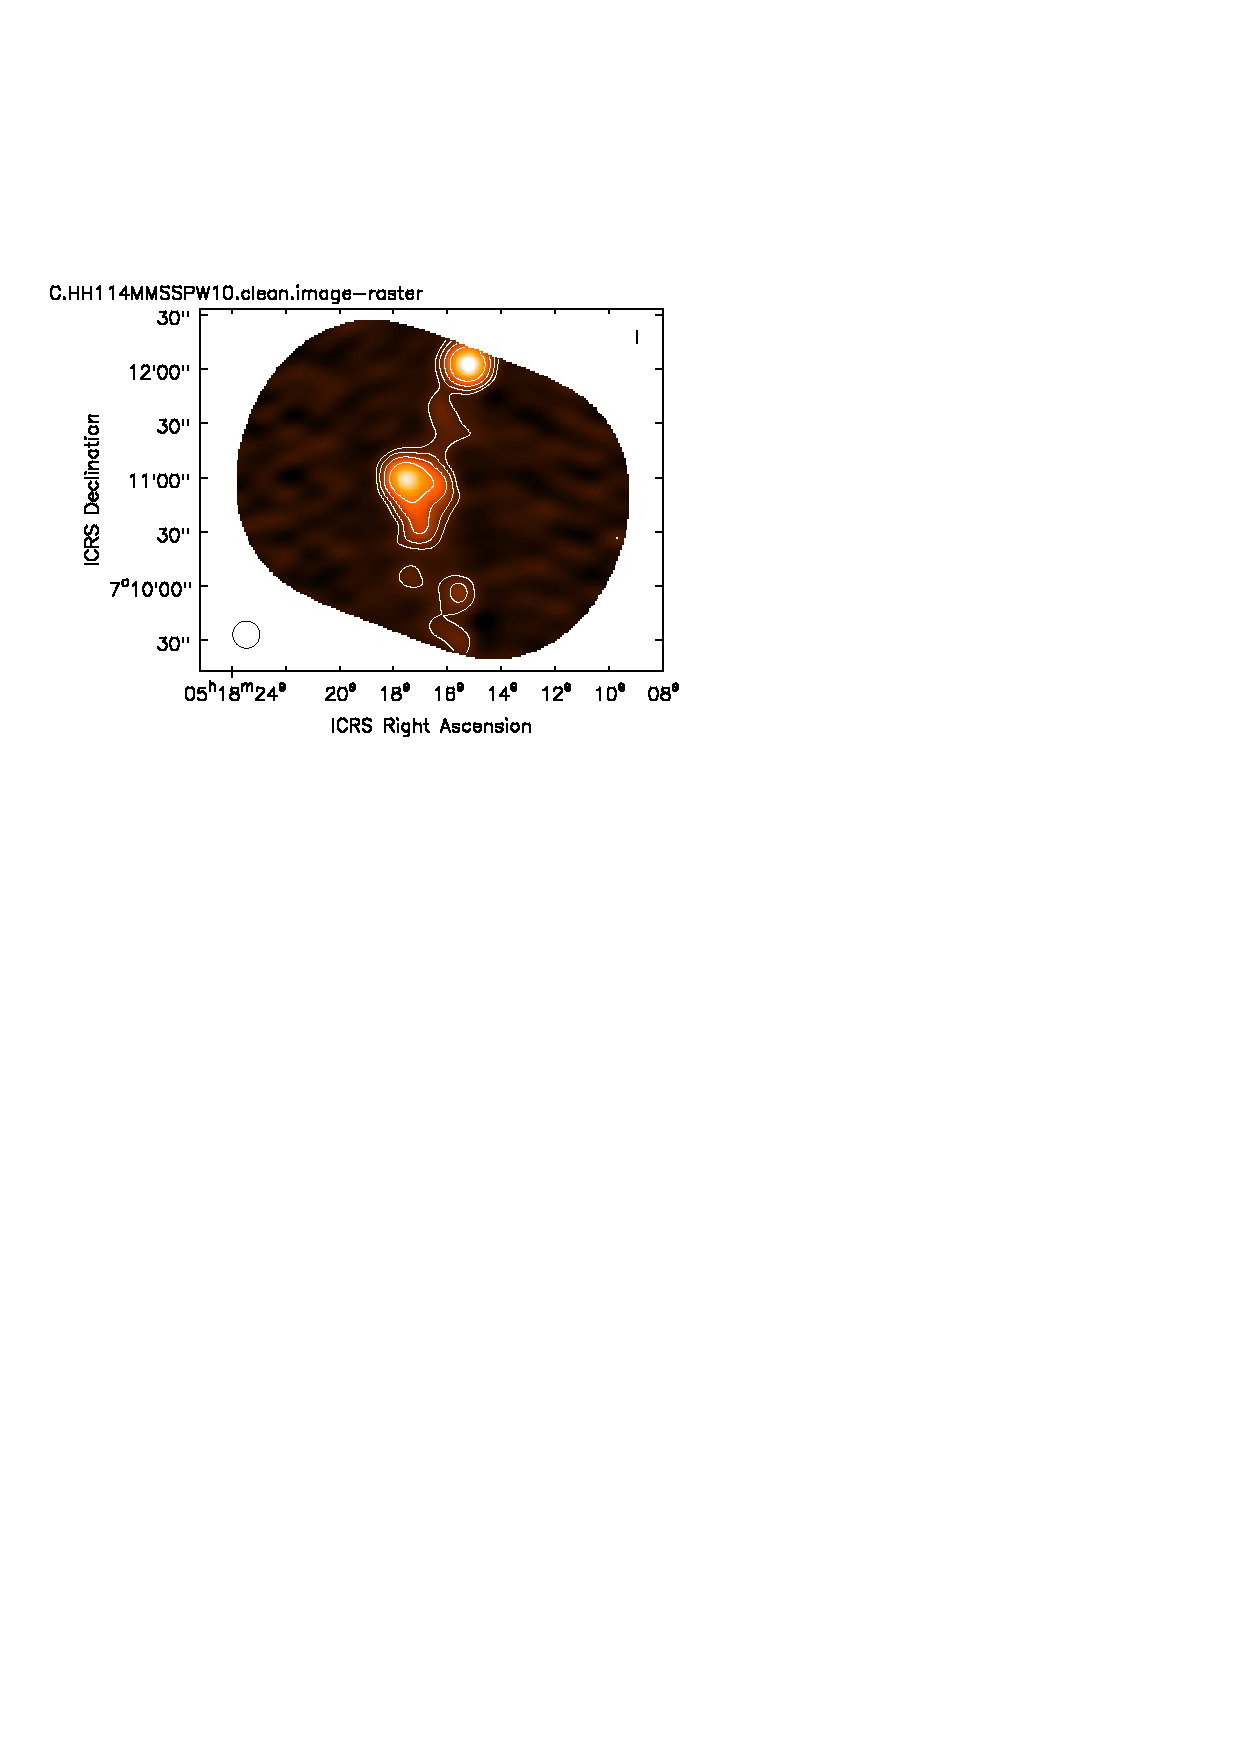
\includegraphics[width=7.5cm]{BLC.HH114MMS.cont.pdf}
	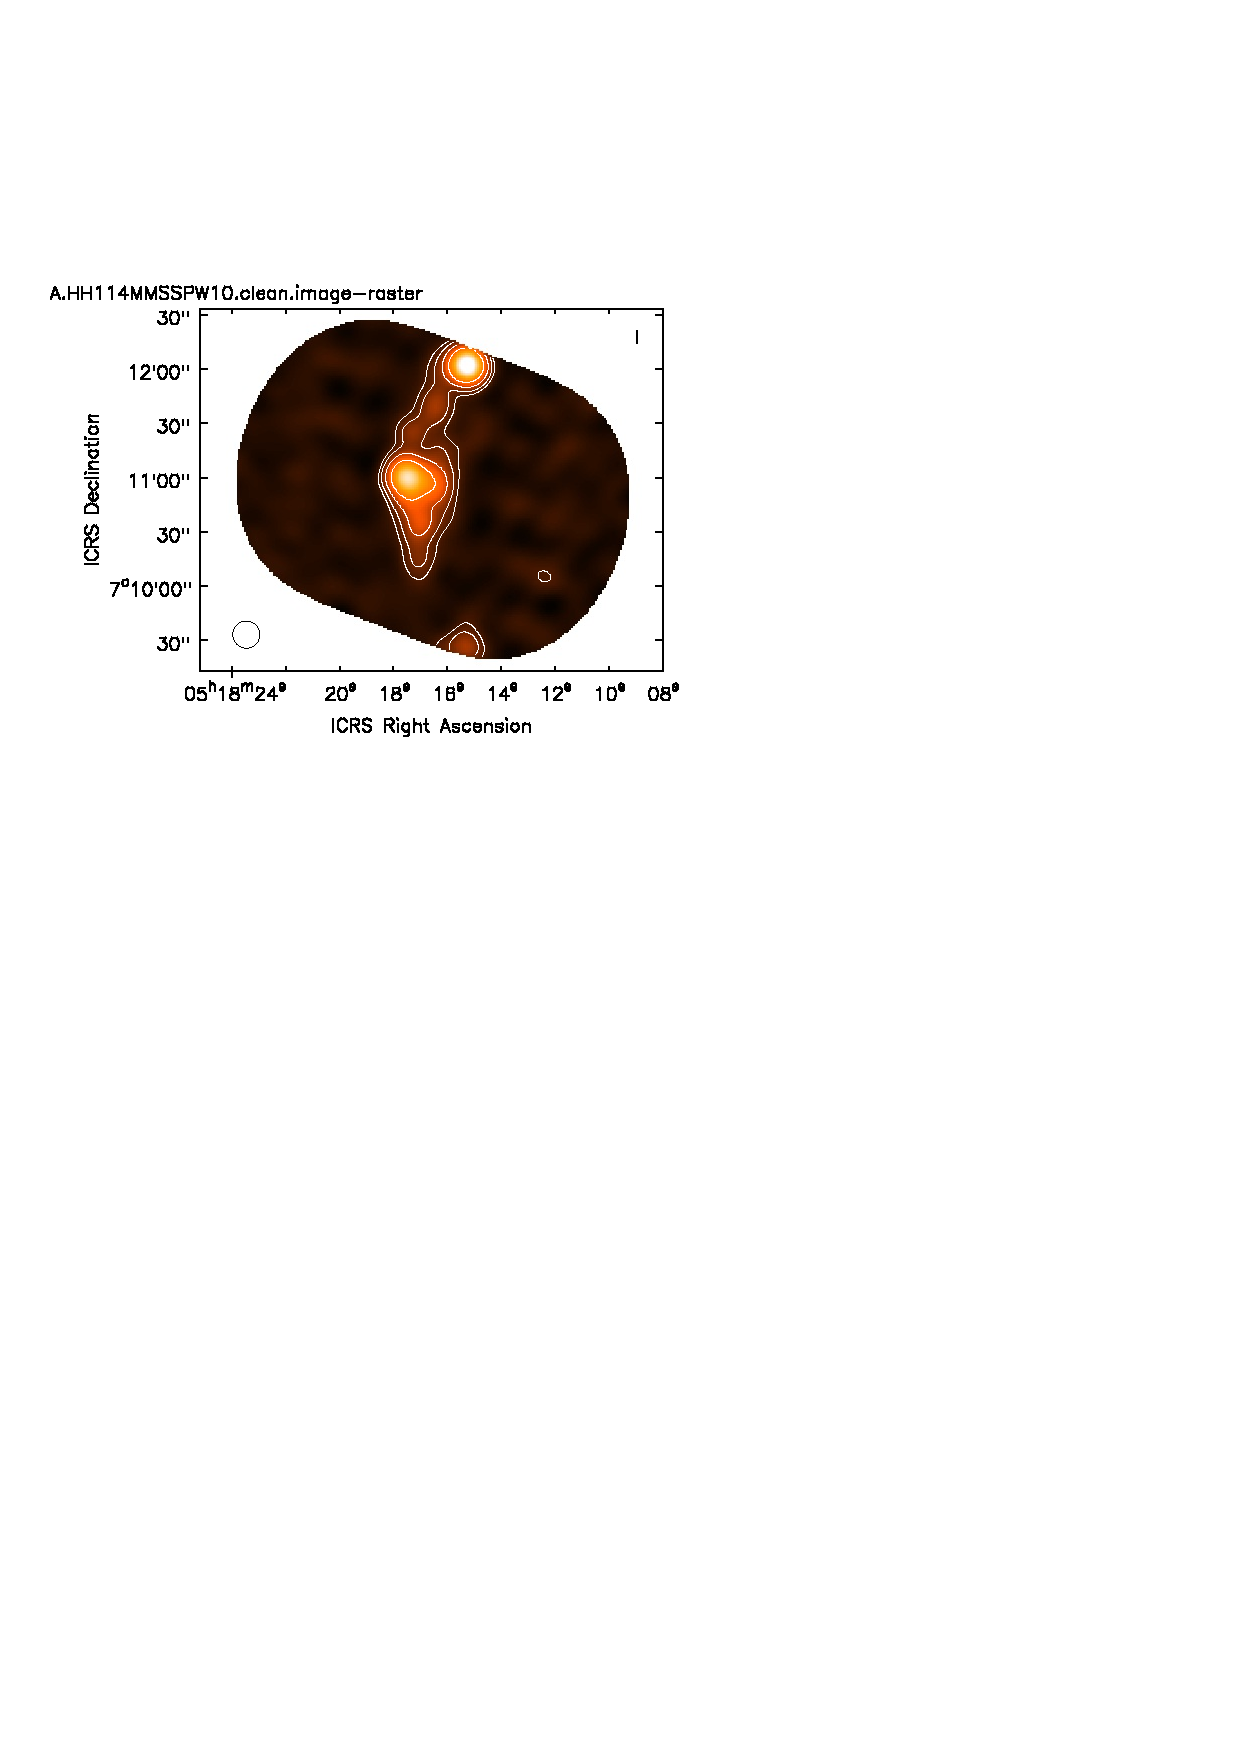
\includegraphics[width=7.5cm]{ACA.HH114MMS.cont.pdf}
	\caption{CLEANed continuum images of HH114MMS correlated with BLC (left) and ACAC (right). CLEAN components are convolved with a $15^{\prime \prime}$ circular restoring beam as presented in the bottom-left corner. Contour levels are $(1, 2, 4, 8) \times 1$ mJy/beam.}\label{fig:contimage}
\end{figure}


\subsection{Spectral lines}\label{subsec:lineimages}
Spectral line images cubes were generated in SPW ID = 2, 4, and 5, where emission lines were significantly detected. Figure \ref{fig:N2H+imageSpec} shows the peak channel image of N$_2$H$^+$ main line correlated with BLC (hot-metal raster image) and ACAC (contour).
Then, we set an integration circle with a radius of 25 pixels centered at (130, 100) (05h18m14s.739, +07º11'18".599) shown as the purple circle, to calculate integrated spectra.

\begin{figure}[h]
	\centering
	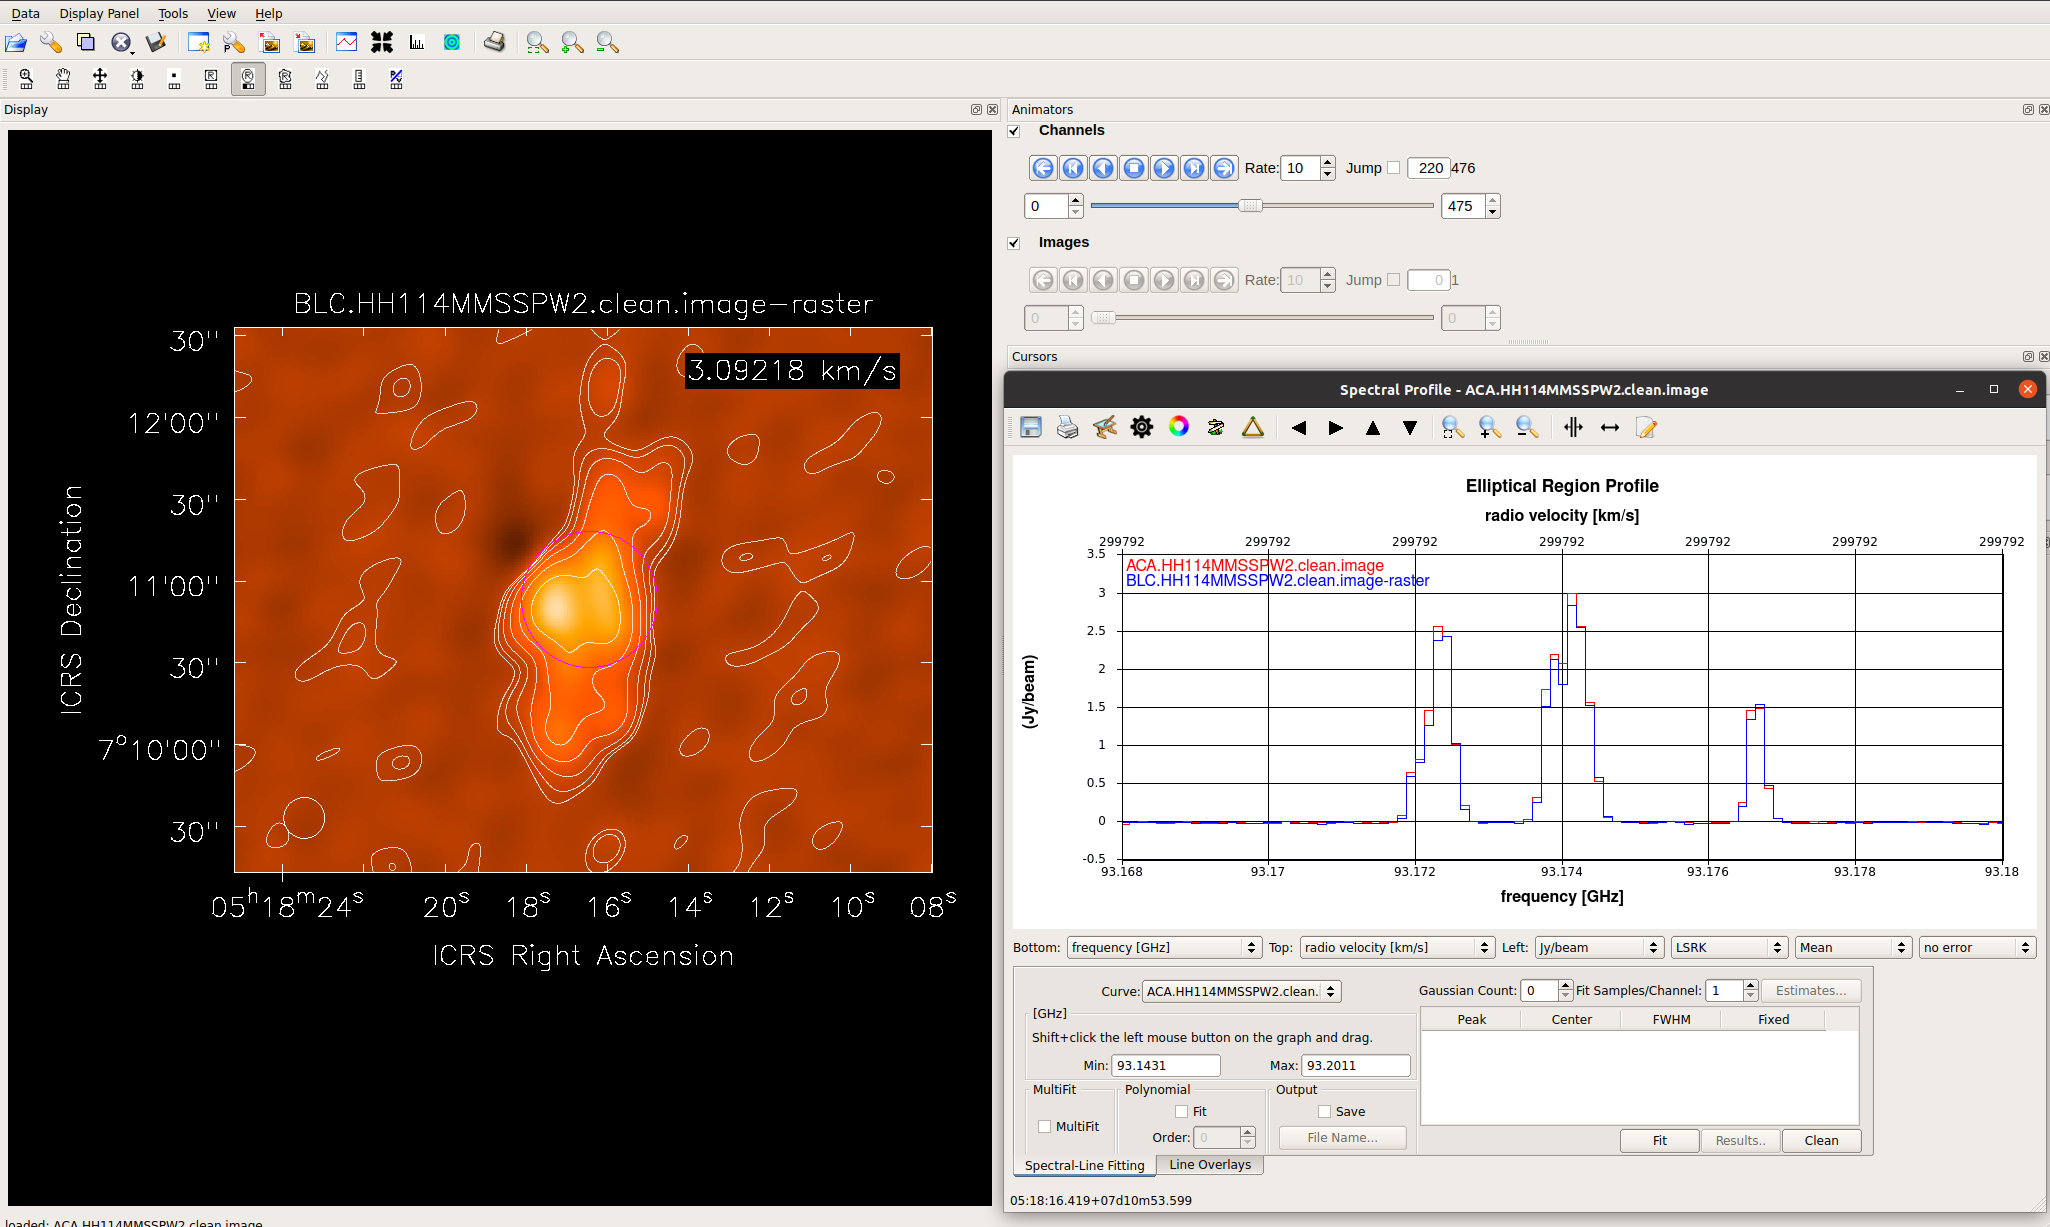
\includegraphics[width=15cm]{HH114MMS-SPW2.png}
	\caption{N$_2$H$^+$ channel map of HH114MMS correlated with BLC (hot-metal raster map) and ACAC (contour). Integrated spectra inside the purple circle are shown in the right panel.}\label{fig:N2H+imageSpec}
\end{figure}

Figures \ref{fig:N2Hspec} shows the integrated line profiles of N$_2$H$^+$, HNC, and HC$_3$N.
Because of differences in channelization between two executions (column 2 in table \ref{tab:Spectra}), we took spline smoothing and resampling to align the spectral channels. 


\begin{figure}[h]
	\centering
	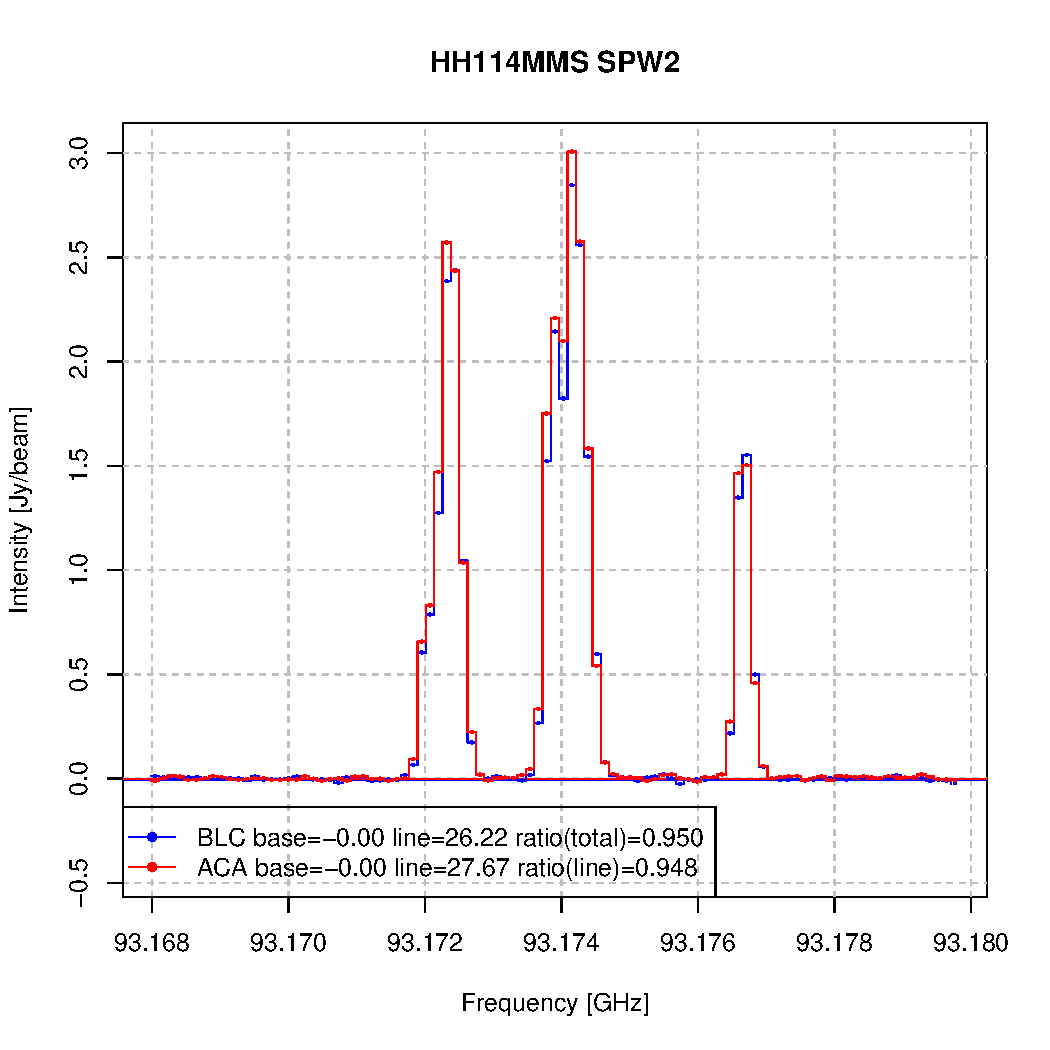
\includegraphics[width=7cm]{HH114MMS.SPW2.pdf}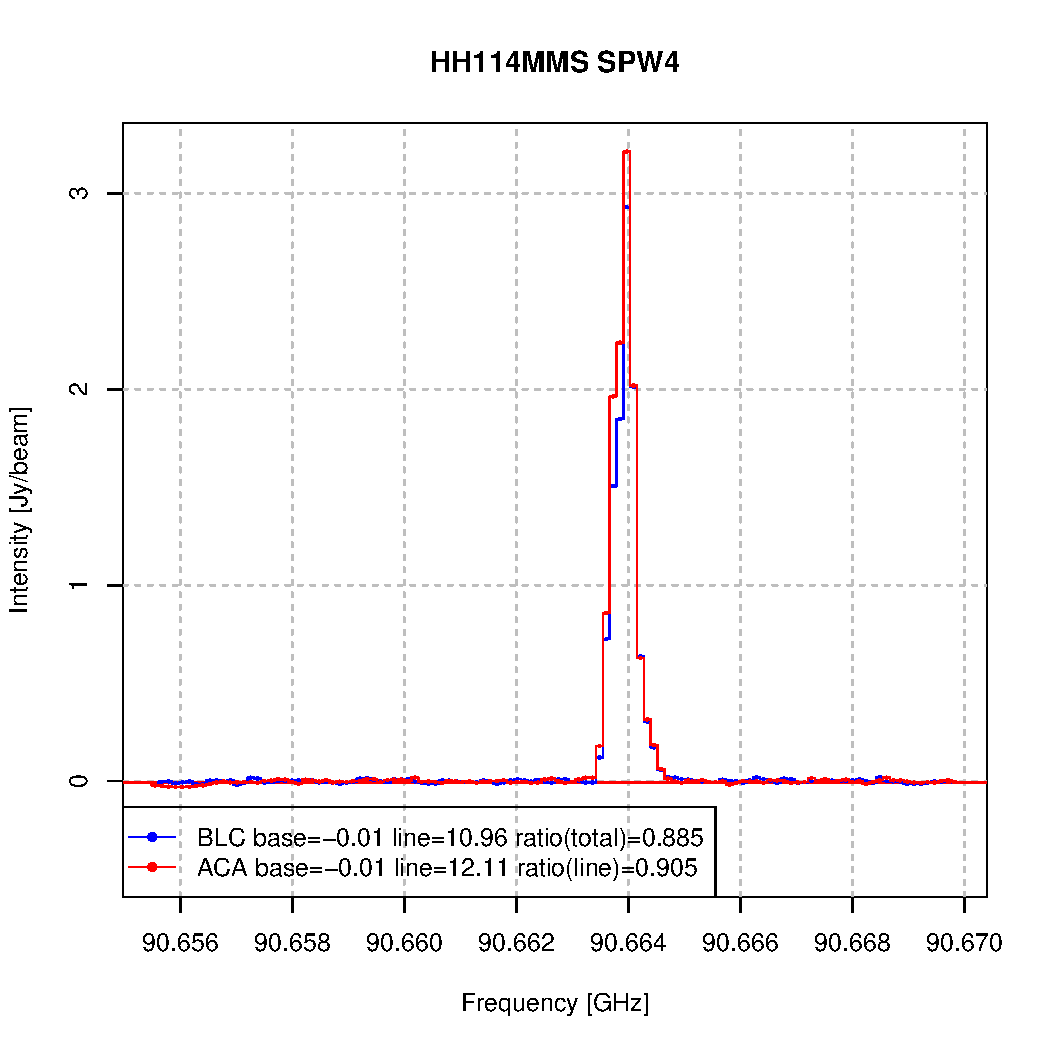
\includegraphics[width=7cm]{HH114MMS.SPW4.pdf}
	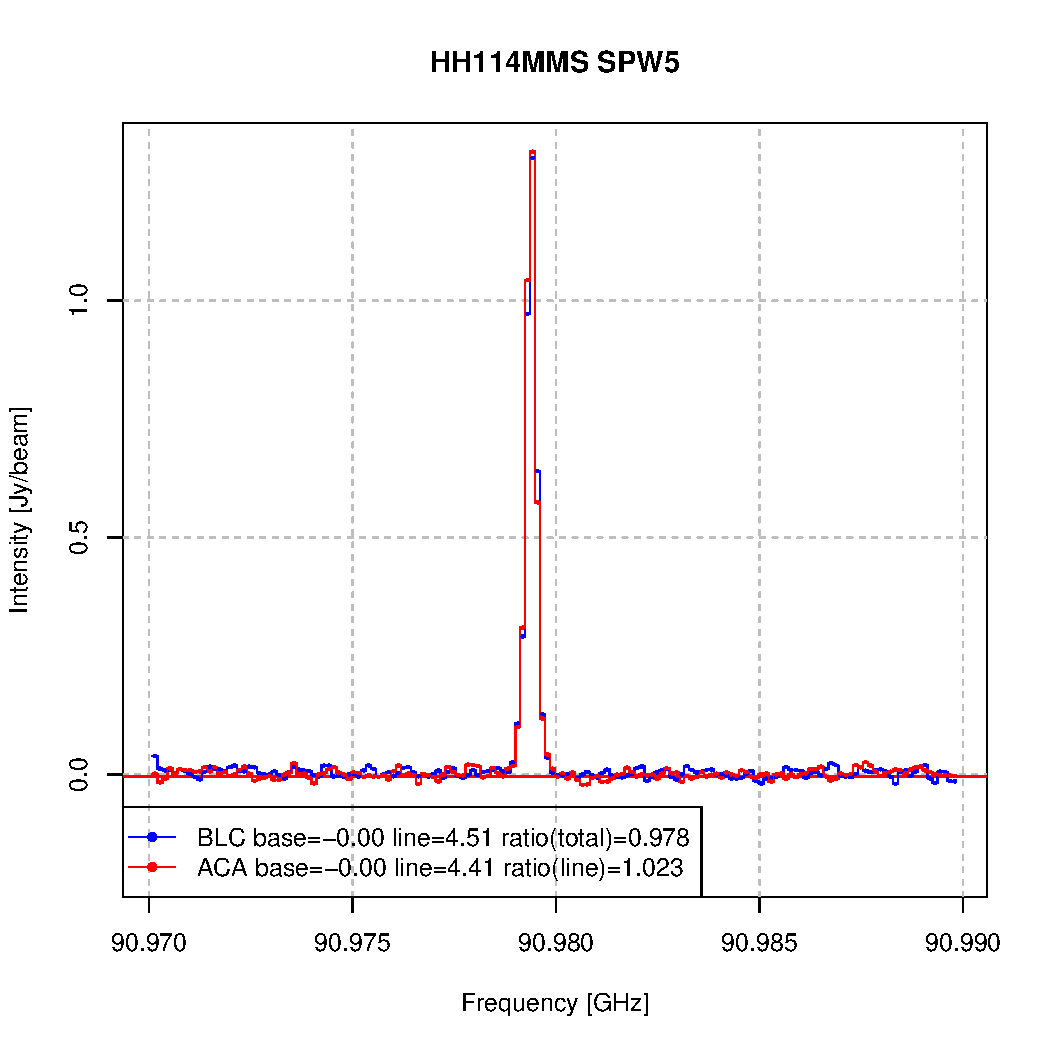
\includegraphics[width=7cm]{HH114MMS.SPW5.pdf}
	\caption{Integrated spectra. (Top left) N$_2$H$^+$ ($\nu_{rest} = 93.1733977$ GHz). Satellite fine structures of $F_1= 1-1$, $F_1 = 0-1$ appear at $\nu_{rest} = 93.17188$ GHz and $\nu_{rest} = 93.17613$ GHz, respectively. (Top right) HNC ($J=1-0$). (Bottom) HC$_3$N ($J=10-9$). Blue and red colors stand for BLC and ACAC data, respectively. Derived ratios are summarized in table \ref{tab:Spectra}.}\label{fig:N2Hspec}
\end{figure}


We have compared the spectra taken with BLC and ACAC by two measures.

\begin{itemize}
\item Total intensity ratio, $R$, obtained by \[ I^\mathrm{BLC}_{\nu} \sim R \cdot I^\mathrm{ACA}_{\nu}, \] where $\sim$ indicates linear regression without intercept.

\item Line flux ratio, $L$, obtained by \[ L = \frac{\sum_{\nu} (I^\mathrm{BLC}_{\nu} - B^\mathrm{BLC}_{\nu})}{\sum_{\nu} (I^\mathrm{ACA}_{\nu} - B^\mathrm{ACA}_{\nu}) }, \] where $B$ is a baseline level shown in the horizontal line in figure \ref{fig:N2Hspec}. The baseline level was determined by percentile of 40\% unless the spectral peak exceeds $2\times$ as high as the median, or 25\% percentile otherwise.
\end{itemize}

These two measures are listed in columns 4 and 5 in table \ref{tab:Spectra}.

\begin{table}[h]
\centering
\caption{Comparison of spectral features}
\label{tab:Spectra}
\begin{tabular}{lcrrr} \hline \hline
Line        & SPW ID & Diff. (ch)  & Intensity Ratio & Line Ratio \\ \hline 
N$_2$H$^+$  & 2      & 0.00        & 0.950           & 0.948 \\
HNC         & 4      & 0.75        & 0.885           & 0.905 \\
HC$_3$N     & 5      & 0.50        & 0.978           & 1.023 \\ \hline
\end{tabular}
\end{table}

\section{Discussion and Summary}
For N$_2$H$^+$ and HC$_3$N lines, integrated line fluxes correlated with BLC and ACAC are consistent within the difference $< 5.2$\%. On the other hand, HNC in SPW ID = 4. shows significantly lower values with BLC, compared with ACAC. This is opposite to the Band-6 results toward G5.89-0.39 and 18089-1732 reported in \href{http://www.alma.cl/~skameno/Documents/CSV-3664/}{CSV-3664 report}, where BLC tended to show greater flux densities especially in very strong emission lines.

For the Band-3 observation in this report, renormalization issue won't account for the difference in HNC profile because the peak flux density of 3.2 Jy is much smaller than the SEFD of $\frac{2 k_B T_{sys}}{A_{e}} \sim 8000$ Jy.
One possible explanation is undersampling of spectral channel for very narrow line profile. The channelization difference of 0.75 ch in this SPW ID (see table \ref{tab:Spectra}) can cause diffrent loss in undersampling.

The results bring up an issue abult frequency mis-alignments in data combining. Since it is difficult to control channel alignments, the spectral resolution must be sufficiently fine compared with the spectral line width.

\end{document}
